\documentclass[11pt,a4paper]{report}
\usepackage[T1]{fontenc}
\usepackage[utf8]{inputenc}
\usepackage{lmodern}
\usepackage[margin=2.5cm]{geometry}
\usepackage{amsmath,amssymb}
\usepackage{booktabs,longtable,array,tabularx}
\usepackage{graphicx}
\usepackage{xcolor}
\usepackage{listings}
\usepackage{microtype}
\usepackage[hidelinks]{hyperref}
\usepackage{caption}
\usepackage{titlesec,fancyhdr,needspace,etoolbox}
\definecolor{navy}{HTML}{14233F}
\definecolor{accent}{HTML}{F47230}
\definecolor{rulegray}{HTML}{C9CED8}
\captionsetup{font=small,labelfont={bf,sf,color=navy},labelsep=period,justification=justified,singlelinecheck=false,skip=6pt}
% chapters run on (no page break) to avoid half-empty pages
\titleclass{\chapter}{straight}
\titleformat{\chapter}[block]{\sffamily\bfseries\huge\color{navy}}{\thechapter}{0.7em}{}[\vspace{2pt}{\color{rulegray}\titlerule[0.8pt]}]
\titlespacing*{\chapter}{0pt}{22pt}{12pt}
\pretocmd{\chapter}{\Needspace{14\baselineskip}}{}{}
\titleformat{\section}{\sffamily\bfseries\Large\color{navy}}{\thesection}{0.6em}{}
\titlespacing*{\section}{0pt}{16pt}{6pt}
\pretocmd{\section}{\Needspace{7\baselineskip}}{}{}
\titleformat{\subsection}{\sffamily\bfseries\large\color{navy}}{\thesubsection}{0.6em}{}
\titlespacing*{\subsection}{0pt}{12pt}{4pt}
\titleformat{\paragraph}[runin]{\sffamily\bfseries\color{navy}}{}{0pt}{}
\titlespacing*{\paragraph}{0pt}{8pt}{0.6em}
% running heads
\pagestyle{fancy}\fancyhf{}
\renewcommand{\chaptermark}[1]{\markboth{\thechapter.\ #1}{}}
\fancyhead[L]{\small\sffamily\color{navy}\leftmark}
\fancyhead[R]{\raisebox{-0.25\height}{
\includegraphics[height=11pt]{figures/dwpc_icon.pdf}}\ \small\sffamily\color{navy}User Manual}
\fancyfoot[C]{\small\sffamily\thepage}
\renewcommand{\headrulewidth}{0.4pt}\renewcommand{\headrule}{{\color{rulegray}\hrule width\headwidth height\headrulewidth}}
\setlength{\headheight}{15pt}
\fancypagestyle{plain}{\fancyhf{}\fancyfoot[C]{\small\sffamily\thepage}\renewcommand{\headrulewidth}{0pt}}
% floats: fewer float-only pages
\renewcommand{\topfraction}{0.9}\renewcommand{\bottomfraction}{0.8}\renewcommand{\textfraction}{0.07}
\renewcommand{\floatpagefraction}{0.85}\setcounter{topnumber}{3}\setcounter{totalnumber}{4}
\setlength{\textfloatsep}{12pt plus 2pt minus 2pt}\setlength{\floatsep}{10pt plus 2pt minus 2pt}
% half-width figure with the caption beside it
\newcommand{\sidefig}[3]{\begin{figure}[!htb]\centering
\begin{minipage}[c]{0.585\textwidth}\includegraphics[width=\linewidth]{#1}\end{minipage}\hfill
\begin{minipage}[c]{0.385\textwidth}\caption{#2}\label{#3}\end{minipage}\end{figure}}

\definecolor{codebg}{HTML}{F6F6F6}
\lstset{basicstyle=\ttfamily\small,backgroundcolor=\color{codebg},frame=none,
        columns=fullflexible,keepspaces=true,showstringspaces=false,
        xleftmargin=0.5em,xrightmargin=0.5em,aboveskip=0.8em,belowskip=0.8em}
\newcommand{\key}[1]{\texttt{\detokenize{#1}}}
\newcommand{\dwpc}{\textsc{dwpc}}
\setlength{\parskip}{0.45em plus 0.1em}
\setlength{\parindent}{0pt}
\emergencystretch=3em
\renewcommand{\arraystretch}{1.15}

\begin{document}
\begin{titlepage}
\newgeometry{margin=2.5cm}
\centering
\vspace*{3.2cm}

\includegraphics[width=0.78\textwidth]{figures/dwpc_logo.pdf}\par
\vspace{1.6cm}
{\color{rulegray}\rule{0.78\textwidth}{0.8pt}}\par\vspace{1.0cm}
{\sffamily\bfseries\fontsize{30}{36}\selectfont\color{navy} User Manual\par}
\vspace{0.5cm}
{\sffamily\large One-dimensional domain-wall dynamics, laser heating\\ and reservoir computing\par}
\vspace{0.9cm}
{\sffamily\normalsize \texttt{laser-thermal} branch\par}
\vfill
{\sffamily\large Razvan-Vasile Ababei\par}
\vspace{0.2cm}
{\sffamily\small RECENT AIR Research Centre, Alexandru Ioan Cuza University of Ia\c{s}i\par}
\vspace{1.2cm}
{\sffamily\small 26 November 2026\par}
\vspace{0.8cm}
{\sffamily\footnotesize\color{black!65} Developers: Razvan-Vasile Ababei and Matt Ellis.\enspace Distributed under the GNU General Public License v3 or later.\par}
\restoregeometry
\end{titlepage}
\tableofcontents

%======================================================================
\chapter{Introduction}

\dwpc{} integrates the equations of motion of one or more magnetic domain walls (DWs), each described by two collective coordinates: its position $x$ along the wire and its tilt angle $\phi$. The wire geometry, the pinning landscape created by notches or anti-notches, applied fields, spin-transfer torque and thermal fluctuations enter as terms of these two equations, so a nanosecond of dynamics takes milliseconds to seconds on one core (Section~\ref{sec:performance}).

What \dwpc{} can do:
\begin{itemize}
\item Driven and stochastic DW dynamics in a polynomial pinning potential (Duffing-like oscillator).
\item Time series, bifurcation diagrams and largest Lyapunov exponents of the DW motion.
\item Reservoir computing with the DW as a nonlinear node (sine/square classification, spoken digits).
\item Several parallel wires whose DWs interact through their stray fields.
\item Temperature-dependent $M_s$, $A$ and pinning, a Gaussian temperature pulse, and a two-temperature model (TTM) for femtosecond laser heating.
\end{itemize}

This manual describes the \texttt{laser-thermal} branch of \url{https://github.com/maxxwave/DWPC}. The temperature features (Chapter~\ref{ch:thermal}), the multi-wire fixes and the cluster scripts exist only on that branch.

Developers: Razvan-Vasile Ababei and Matt Ellis (University of Sheffield, 2019); laser and thermal extension by Razvan-Vasile Ababei, UAIC Ia\c{s}i, 2026. \dwpc{} is distributed under the GNU General Public License, version~3 or later. The model, the Ni anti-notch potential and its use for reservoir computing are described in Ababei \emph{et al.}, Sci.\ Rep.\ \textbf{11}, 15587 (2021)~\cite{ababei2021}, and the atomistic origin of the bistable dynamics in double-notched Ni nanowires in Ref.~\cite{ababei2026}. Please cite Ref.~\cite{ababei2021} when you use \dwpc.

%======================================================================
\chapter{Installation and running}

\section{Compilation}
\dwpc{} needs Linux (or WSL), a C++11 compiler and LAPACK (used by the reservoir-computing readout and linked by every build).
\begin{lstlisting}
sudo apt-get install g++ liblapack-dev
git clone -b laser-thermal https://github.com/maxxwave/DWPC.git
cd DWPC
make            # builds the executable ./DWPC
\end{lstlisting}
\begin{itemize}
\item The README of \texttt{master} mentions \texttt{sh makefile.sh}; the build file is \texttt{makefile}, so the command is \texttt{make}.
\item The makefile compiles with \texttt{-O3 -g -pg}. \texttt{-pg} (profiling) slows the run slightly and writes \texttt{gmon.out} in the run directory; remove it for production runs.
\item The makefile does not track headers: after editing a file in \texttt{hdr/}, rebuild everything (\texttt{touch src/*.cpp; make}).
\item \dwpc{} is serial. Ensembles run as independent jobs; the \texttt{cluster/} folder has Slurm job arrays and deploy/collect scripts (Section~\ref{sec:cluster}).
\end{itemize}

\section{The input file}
A run is defined entirely by the plain-text file \texttt{input} in the working directory; all quantities are in SI units. Run \dwpc{} from that directory, \texttt{/path/to/DWPC/DWPC > log}; output files are written to the current directory, so use one directory per run. The parser follows these rules:
\begin{itemize}
\item One \key{key=value} per line. Keys are case-sensitive; only the first token after \texttt{=} is read, so \texttt{H=990 \#A/m} gives 990.
\item Lines starting with \texttt{\#} are ignored. If a key appears twice, the last line wins.
\item A key the code asks for but the file lacks prints \texttt{Warning: Input key not found} and takes its default (Chapter~\ref{ch:keywords}). Keys without a default fall back to 0: a missing \key{Ms}, \key{Lz} or \key{Dt} makes the run meaningless, so always check the warnings at the top of the log.
\item Keys the code never reads are ignored silently (for example \key{pin} in the shipped example).
\end{itemize}

The smallest useful input, a single DW driven by an oscillating field at 100~K:
\begin{lstlisting}
Ms=477e3
L=400e-9
Ly=50e-9
Lz=5e-9
Aex=1.05e-11
alpha=0.02
Nwires=1
a2=-1.2866e-6
a4=1.632e8
H=990
f=500e6
Temperature=100
P=0.7
beta=0.04
j=0
Dt=1e-13
totaltime=20e-9
out_time=1e-10
integrator=RK4
program=Benchmark2
\end{lstlisting}
\key{program} selects what \dwpc{} does (Chapter~\ref{ch:programs}). At start-up \dwpc{} prints every parameter it uses, the derived quantities (demagnetising field, DW width, critical current) and, if enabled, the temperature model. Read this header first: it is the record of what was actually simulated.

%======================================================================
\chapter{Physics: the one-dimensional DW model}\label{ch:model}

A transverse DW in a strip of width $L_y$ and thickness $L_z$ (cross-section $S=L_yL_z$) is treated as a rigid object with two degrees of freedom: its centre $x$ and the angle $\phi$ of its magnetisation out of the strip plane. These are the collective coordinates of the $q$--$\phi$ model of Malozemoff and Slonczewski~\cite{malozemoff}, extended with spin-transfer torque by Thiaville \emph{et al.}~\cite{thiaville}.

\section{Equations of motion}
With $\gamma'=\gamma/(1+\alpha^2)$ and $\gamma=1.76\times10^{11}$~T$^{-1}$s$^{-1}$, \dwpc{} integrates
\begin{align}
\dot\phi &= -\frac{\gamma'}{2M_sS}\frac{\partial E}{\partial x} - \frac{\alpha\gamma'\mu_0H_K}{2}\sin2\phi + \gamma'\mu_0H(t) + (\beta-\alpha)\frac{u}{\Delta}, \label{eq:phi}\\
\dot x &= \frac{\gamma\mu_0H_K}{2}\,\Delta\sin2\phi + \alpha\Delta\dot\phi + u, \label{eq:x}
\end{align}
plus the thermal terms of Section~\ref{sec:noise}. $E(x)$ is the pinning energy, $H(t)$ the applied field along the wire, $u$ the spin-drift velocity, $\alpha$ the Gilbert damping and $\beta$ the non-adiabatic parameter.

\section{Demagnetising field and DW width}
The hard-axis field $H_K=M_s(N_z-N_y)$ uses the demagnetising factors of an infinitely long rectangular prism~\cite{aharoni}:
\begin{equation}
N_y = 1-\frac{2}{\pi}\arctan\frac{L_y}{L_z}+\frac{L_z}{2\pi L_y}\ln\!\left(1+\frac{L_y^2}{L_z^2}\right)-\frac{L_y}{2\pi L_z}\ln\!\left(1+\frac{L_z^2}{L_y^2}\right),\qquad N_z=1-N_y .
\end{equation}
For $50\times5$~nm this gives $N_y=0.1211$, $N_z=0.8789$ and $H_K=0.758\,M_s$ (verified in Section~\ref{sec:demag}). Versions before commit \texttt{dd3d90c} used $\log_{10}$ here and overestimated $H_K$ by 8.6\%.

The DW width follows the angle $\phi$ (Pivano--Dolocan form~\cite{pivano}):
\begin{equation}
\Delta(\phi)=\pi\sqrt{\frac{2A}{K_{\rm eff}(\phi)}},\qquad K_{\rm eff}(\phi)=\mu_0M_s^2\sin^2\phi+\mu_0M_sH_K .
\end{equation}
The factor $\pi$ makes $\Delta$ a full wall width rather than the Bloch parameter used in textbook Walker formulas; keep this in mind when comparing velocities with analytic results.

\section{Pinning potential}
The notches or anti-notches enter as a polynomial energy $E(x)=\sum_{n=0}^{8}a_nx^n$ (J), fitted to micromagnetic simulations of the real geometry. The force uses only the even part,
\begin{equation}
\frac{\partial E}{\partial x}=2a_2x+4a_4x^3+6a_6x^5 ,
\end{equation}
so $a_1,a_3,a_5,a_7,a_8$ are read but have no effect: the potential is symmetric. With $a_2<0$ and $a_4>0$ it is a double well with minima at $x_0=\pm\sqrt{-a_2/2a_4}$ and barrier $a_2^2/4a_4$; the shipped Ni values give $\pm63$~nm and $2.5\times10^{-21}$~J ($0.6\,k_BT$ at 300~K). With \key{pinning_exponent}~$=p$ the energy is scaled by $(M_s(T)/M_s(T_0))^p$ (Chapter~\ref{ch:thermal}).

\section{Applied field and edge roughness}
\begin{equation}
H(t,x)=H_0\sin(2\pi ft)+H_{\rm const}+H_{\rm edge}(x).
\end{equation}
$H_{\rm const}$ is applied only for $t<25$~ns (hard-coded). Edge roughness (\key{use_edge_roughness=1}) divides the wire into segments of length \key{edge_scale}; segment $j$ carries the field $H_{\rm edge,max}(U_j-U_{j+1})$ with $U_j$ uniform random numbers in $[0,1)$, reproducible through \key{edge_seed}.

\section{Spin-transfer torque}
A current density $j$ gives the spin-drift velocity $u=jP\mu_B/(eM_s)$ with polarisation $P$, entering as the adiabatic term $u$ and the non-adiabatic term $(\beta-\alpha)u/\Delta$. \textbf{Note:} \texttt{calculate::current()} multiplies \texttt{stor::j\_dens} by its argument, so a single DW sees $j^2$ in place of $j$. This needs checking before any current-driven study; with the default $j=0$ it has no effect.

\section{Thermal fluctuations}\label{sec:noise}
Thermal noise enters as Gaussian random terms on $\phi$ and $x$ whose amplitude follows the fluctuation--dissipation theorem~\cite{brown}:
\begin{equation}
\sigma=\sqrt{\frac{\alpha k_BT\gamma'}{M_sS\Delta\,\Delta t}},\qquad \delta\dot\phi=\sigma n_\phi,\qquad \delta\dot x=\sigma\Delta n_x ,
\end{equation}
with $n_\phi,n_x$ independent standard normal numbers drawn once per time step and used in every stage of the stochastic Heun or Runge--Kutta step. $T$ is the spin temperature: the constant \key{Temperature}, or $T(t)$ from Chapter~\ref{ch:thermal}. Section~\ref{sec:equipartition} checks that this amplitude reproduces equipartition. The generator is \texttt{std::default\_random\_engine}, seeded from the clock or from \key{rng_seed}.

%======================================================================
\chapter{Physics: coupling between DWs in neighbouring wires}\label{ch:coupling}

With \key{Nwires}~$>1$ and \key{use_DW_coupling=1}, the wires lie side by side in the plane with an edge-to-edge gap \key{rij}, so neighbouring DWs are a centre distance $d=r_{ij}+L_y$ apart across the wires. A head-to-head or tail-to-tail DW carries a net magnetic charge $q=2M_sS$, and to first order DWs in adjacent wires interact like point charges (Coulomb-like potential~\cite{hayward}). \dwpc{} adds the stray field of each nearest neighbour $j$ to the field acting on DW $i$:
\begin{equation}
H_i=H(t)-H_i^{\rm mono}-H_i^{\rm dd},\qquad H_i^{\rm mono}=-\sum_{j=i\pm1}\frac{M_sS\,(x_i-x_j)}{2\pi r_{ij}^3},\qquad r_{ij}^2=(x_i-x_j)^2+d^2 .
\end{equation}
The monopole term is the field $q/(4\pi r^2)$ of the neighbour's charge projected on the wire axis. A second term treats the transverse moment of each wall, $m_y=7.1\times10^{-18}$~A\,m$^2$ (constant in the code), as a point dipole:
\begin{equation}
H_i^{\rm dd}=\sum_{j=i\pm1}\frac{3m_y^2}{8\pi M_sS}\,\frac{(x_i-x_j)\left[(x_i-x_j)^2-4d^2\right]}{r_{ij}^7}.
\end{equation}

Consequences that are useful to know:
\begin{itemize}
\item Equal charges (all walls head-to-head) repel; Figure~\ref{fig:coupling} shows two walls separating without pinning or field at 0~K.
\item Exactly aligned walls feel no force: they sit on an unstable equilibrium and stay there at 0~K. Any offset, or thermal noise at $T>0$, breaks the symmetry and grows.
\item The interaction energy for a 100~nm relative displacement drops from about $4\,k_BT$ (300~K) at $d=100$~nm to $0.7\,k_BT$ at 200~nm and $0.1\,k_BT$ at 400~nm.
\item Only nearest neighbours interact. For small offsets, the field from the second neighbour would be about 1/8 of the first.
\end{itemize}

The point-charge picture is qualitatively correct at all spacings, but O'Brien \emph{et al.}~\cite{obrien} showed that near-field interactions (spacings below the DW size, about 100~nm in Permalloy) need the full charge distribution inside the wall, and that a point-like description cannot reproduce them. Treat \dwpc{} as quantitative only for centre distances of several wire widths, and check smaller spacings against MuMax3 or VAMPIRE.

%======================================================================
\chapter{Physics: temperature and laser heating}\label{ch:thermal}

\section{Temperature-dependent parameters}
With \key{use_Ms_T=1} the saturation magnetisation follows the rescaled form used by Evans, Atxitia and Chantrell to map classical atomistic $M(T)$ curves onto experiment~\cite{evans2015}:
\begin{equation}
M_s(T)=M_{s0}\left[1-\left(\frac{T}{T_c}\right)^{a}\right]^{\beta},\qquad T<T_c .
\end{equation}
\key{Ms} in the input is then $M_{s0}$ (0~K), \key{Ms_exponent} is $\beta$ and \key{Ms_rescaling_exponent} is $a$ (1 = classical form). For Ni, Evans \emph{et al.} give $T_c=635$~K, $\beta=0.341$ and $a=2.322$. Two optional scalings follow $M_s$:
\begin{equation}
A(T)=A_0\left(\frac{M_s(T)}{M_{s0}}\right)^{n},\qquad E_{\rm pin}(x,T)=E_{\rm pin}(x)\left(\frac{M_s(T)}{M_s(T_0)}\right)^{p},
\end{equation}
with $n=$~\key{Aex_exponent} (\key{Aex} is then $A_0$) and $p=$~\key{pinning_exponent}; the pinning polynomial is taken to be fitted at the base temperature $T_0=$~\key{Temperature}. With $n=p=2$ every micromagnetic energy scales as $M_s^2$, so the DW width stays constant and the ratio of pinning to inter-wire coupling does not change with temperature. Exponents from atomistic calculations are smaller than 2 (around 1.7--1.8 for FePt), so use VAMPIRE values where available.

Every quantity that depends on $M_s$ ($\mu_0M_s$, $H_K$, the four prefactors of Eqs.~\eqref{eq:phi}--\eqref{eq:x}, $A$ and the pinning scale) is recomputed whenever $M_s$ changes, at every stage of every time step when $T$ depends on time.

\section{Gaussian temperature pulse}
The simplest time-dependent case (\key{use_T_pulse=1}):
\begin{equation}
T(t)=T_0+\Delta T\exp\!\left[-\frac{(t-t_0)^2}{2\sigma^2}\right].
\end{equation}
The run stops if $T_0+\Delta T\ge T_c$ while \key{use_Ms_T=1}.

\section{Two-temperature model}\label{sec:ttm}
A femtosecond pulse heats the electrons first; they pass energy to the lattice through the electron--phonon coupling $G$. With \key{use_TTM=1} \dwpc{} integrates
\begin{align}
\gamma_eT_e\frac{dT_e}{dt}&=-G(T_e-T_l)+P_0\exp\!\left[-\frac{(t-t_0)^2}{2\sigma^2}\right],\\
C_l\frac{dT_l}{dt}&=G(T_e-T_l)-C_l\frac{T_l-T_0}{\tau_{\rm cool}} .
\end{align}
The electron heat capacity is $C_e=\gamma_eT_e$; the last term removes heat to the substrate and is switched off by \key{TTM_tau_cool=0}. The pulse is given either as the peak absorbed power density $P_0$ or as the absorbed fluence $F$, assumed uniform over the thickness: $P_0=F/(L_z\sigma\sqrt{2\pi})$. For Ni, Beaurepaire \emph{et al.}~\cite{beaurepaire} used $\gamma_e=6\times10^3$~J\,m$^{-3}$K$^{-2}$ and $G=8\times10^{17}$~W\,m$^{-3}$K$^{-1}$ on a 22~nm film pumped with 60~fs pulses of 7~mJ/cm$^2$.

\begin{sloppypar}The spin temperature $T_s$ that sets $M_s(T)$ and the thermal noise is $T_e$ (\key{TTM_spin_temperature=electron}, default) or $T_l$ (\key{phonon}). $M_s$ either follows $M_s(T_s)$ instantly or, with \key{TTM_tau_m}~$>0$, relaxes towards it with a finite time:\end{sloppypar}
\begin{equation}
\frac{dm}{dt}=\frac{m_{\rm eq}(T_s)-m}{\tau_m},\qquad M_s=m\,M_{s0}.
\end{equation}
This relaxation is phenomenological: calibrate $\tau_m$ against atomistic $m(t)$ for the same pulse. When $T_e$ exceeds $T_c$, instantaneous $M_s$ drops to zero and the 1D model is no longer defined; \dwpc{} stops with an explanation if $M_s$ falls below 0.1\% of $M_{s0}$, and a finite $\tau_m$ keeps $M_s$ positive through short excursions above $T_c$.

Numerically, the TTM runs with its own adaptive RK4 sub-steps (limited by the electron--phonon, lattice, cooling and $\tau_m$ times, by $\sigma/20$ within $8\sigma$ of the pulse, and by \key{TTM_dt_max}) and keeps a short history of states, so every stage of the DW integrator gets the temperatures at its exact time. A run that restarts time at 0 (for example \key{Bifurcation}) integrates the TTM again from the start.

%======================================================================
\chapter{Numerical methods}\label{ch:numerics}

\section{Integrators}
All integrators use the fixed step \key{Dt}; \key{out_time} sets how often a line is written. Only HEUN and RK4 add thermal noise.

\begin{center}\small
\begin{tabularx}{\textwidth}{@{}l l l X@{}}
\toprule
\key{integrator} & Deterministic order & Thermal noise & Use \\
\midrule
\key{RK4} & 4 & yes & default; single and multi-wire runs \\
\key{HEUN} & 2 & yes & stochastic runs, cheaper per step \\
\key{RK45} & 5 (fixed step) & no & deterministic dynamics, Lyapunov, bifurcation \\
\key{EULER} & --- & no & not usable \\
\bottomrule
\end{tabularx}
\end{center}
The orders are measured in Section~\ref{sec:convergence}. \key{RK45} returns an embedded error estimate but does not use it for step control. \key{Benchmark3} (coupled wires) accepts only \key{RK4}.

Choosing \key{Dt}:
\begin{itemize}
\item Without a laser pulse, 0.1~ps resolves the DW precession and GHz driving; RK4 is converged to the round-off floor already at 1--2~ps (Figure~\ref{fig:convergence}).
\item With the TTM the temperature has its own sub-steps, but the DW equations see $M_s$ change on the pulse time scale; use \key{Dt} well below the pulse width (for example 0.05~fs for a 50--60~fs pulse).
\item The noise amplitude grows as $1/\sqrt{\Delta t}$ by construction, so $x(t)$ and $\phi(t)$ look noisier at small \key{Dt}; average over realisations, not over shorter steps.
\item The step counter is an \texttt{int}: \key{totaltime}/\key{Dt} must stay below about $2\times10^9$ steps.
\end{itemize}

\section{Reproducibility}
The noise generator is seeded from the clock unless \key{rng_seed}~$>0$. Runs with the same seed and the same sequence of random draws are bit-identical, which allows paired comparisons: the same noise with and without a laser pulse (Section~\ref{sec:cluster}). \key{edge_seed} reseeds the generator only while building the edge-roughness field.

\section{Largest Lyapunov exponent}
\key{program=Lyapunov} integrates two trajectories, from $x=0$ and from $x=0.1$~nm, stores $x$ at every output time, and averages $\ln(|\delta x(t)|/|\delta x_0|)/N_{\rm out}$ over the run. The separation is not renormalised, so the estimate is only meaningful while $\delta x$ is small compared with the size of the attractor; use RK45 (no noise) for a deterministic exponent. \texttt{calculate::Jacobian} provides the Jacobian of the deterministic flow for tangent-space methods.

\section{Reservoir computing}
The DW acts as a nonlinear node with time multiplexing~\cite{ababei2021}: each input value sets the amplitude of the driving field for a node time $\theta=T/N_v$, and the RMS DW position over that time is the node state. A linear readout is trained by ridge regression (LAPACK). The two tasks shipped with the code, sine/square classification and spoken digit recognition, are described in Chapter~\ref{ch:rc}; their settings are read from the separate file \texttt{rc\_input} (Section~\ref{sec:rcinput}).

%======================================================================
\chapter{Input keyword reference}\label{ch:keywords}

Every key read from \texttt{input} on the \texttt{laser-thermal} branch. A dash in the default column means the key has no default and falls back to 0 with a warning.

\newcommand{\kwtable}[1]{{\small\begin{longtable}{@{}>{\raggedright}p{4.0cm} >{\raggedright}p{1.9cm} >{\raggedright}p{2.6cm} >{\raggedright\arraybackslash}p{6.0cm}@{}}\toprule Key & Unit & Default & Meaning\\\midrule\endhead #1\bottomrule\end{longtable}}}

\section{Material and geometry}
\kwtable{
\key{Ms} & A/m & --- & saturation magnetisation ($M_{s0}$ at 0 K when \key{use_Ms_T=1})\\
\key{Aex} & J/m & --- & exchange stiffness ($A_0$ at 0 K when \key{Aex_exponent}~$\neq0$)\\
\key{alpha} & --- & --- & Gilbert damping\\
\key{L} & m & --- & wire length (edge-roughness segments)\\
\key{Ly} & m & --- & wire width\\
\key{Lz} & m & --- & wire thickness\\}

\section{Pinning potential}
\kwtable{
\key{a0}\ldots\key{a8} & J/m$^n$ & $a_2=-1.29\times10^{-7}$, $a_4=1.632\times10^8$, others 0 & coefficients of $E(x)=\sum a_nx^n$; only $a_2,a_4,a_6$ enter the force\\
\key{use_edge_roughness} & --- & 0 & 1 adds a random piecewise-constant edge field\\
\key{H_edge_max} & A/m & 0 & amplitude of the edge field\\
\key{edge_scale} & m & $2\times10^{-8}$ & segment length of the edge field\\
\key{edge_seed} & --- & 0 & seed for the edge field (0 = current generator state)\\}

\section{Applied field and spin current}
\kwtable{
\key{H} & A/m & --- & amplitude $H_0$ of the oscillating field\\
\key{f} & Hz & --- & frequency of the field\\
\key{H_const} & A/m & 0 & constant field, applied for $t<25$ ns\\
\key{j} & A/m$^2$ & --- & current density (see the note in Chapter~\ref{ch:model})\\
\key{P} & --- & --- & spin polarisation\\
\key{beta} & --- & --- & non-adiabatic parameter\\}

\section{Simulation control}
\kwtable{
\key{program} & --- & \key{Benchmark2} & what to run (Chapter~\ref{ch:programs})\\
\key{integrator} & --- & \key{RK4} & \key{RK4}, \key{HEUN}, \key{RK45} or \key{EULER}\\
\key{Dt} & s & --- & time step\\
\key{totaltime} & s & --- & simulated time\\
\key{out_time} & s & --- & output interval\\
\key{Temperature} & K & --- & temperature; base temperature $T_0$ with a pulse or the TTM\\
\key{rng_seed} & --- & 0 & fixed noise seed; 0 seeds from the clock\\}

\section{Several wires}
\kwtable{
\key{Nwires} & --- & --- & number of wires (DWs)\\
\key{use_DW_coupling} & --- & 0 & 1 switches on the inter-wire stray fields\\
\key{rij} & m & $5\times10^{-8}$ & edge-to-edge gap; centre distance = \key{rij} + \key{Ly}\\
\key{DW_x0_<i>} & m & 10 nm (wires 0, 1), 87.05 nm (others) & initial DW position in wire $i$\\
\key{DW_phi0_<i>} & rad & 0 & initial DW angle in wire $i$\\}

\section{Temperature-dependent parameters}
\kwtable{
\key{use_Ms_T} & --- & 0 & 1 enables $M_s(T)$\\
\key{Tc} & K & 0 & Curie temperature (must be $>0$)\\
\key{Ms_exponent} & --- & 0 & $\beta$ (must be $>0$)\\
\key{Ms_rescaling_exponent} & --- & 1 & $a$ in $(T/T_c)^a$\\
\key{Aex_exponent} & --- & 0 & $n$ in $A\propto M_s^n$\\
\key{pinning_exponent} & --- & 0 & $p$ in $E_{\rm pin}\propto M_s^p$\\}

\section{Temperature pulse and two-temperature model}
\kwtable{
\key{use_T_pulse} & --- & 0 & Gaussian $T(t)$ (not with \key{use_TTM})\\
\key{T_pulse_peak} & K & 0 & peak rise $\Delta T$\\
\key{T_pulse_t0} & s & 0 & time of the maximum\\
\key{T_pulse_sigma} & s & 0 & standard deviation (must be $>0$)\\
\key{use_TTM} & --- & 0 & two-temperature model (needs \key{Temperature}~$>0$)\\
\key{TTM_gamma_e} & J\,m$^{-3}$K$^{-2}$ & 0 & electron heat capacity coefficient\\
\key{TTM_C_l} & J\,m$^{-3}$K$^{-1}$ & 0 & lattice heat capacity\\
\key{TTM_G} & W\,m$^{-3}$K$^{-1}$ & 0 & electron--phonon coupling\\
\key{TTM_P0} & W\,m$^{-3}$ & 0 & peak absorbed power density\\
\key{TTM_fluence} & J\,m$^{-2}$ & 0 & absorbed fluence, alternative to \key{TTM_P0}\\
\key{TTM_t0} & s & 0 & time of the pulse maximum\\
\key{TTM_sigma} & s & 0 & pulse standard deviation; FWHM $=2.355\sigma$\\
\key{TTM_tau_cool} & s & 0 & lattice cooling time; 0 = off\\
\key{TTM_tau_m} & s & 0 & magnetisation relaxation time; 0 = instantaneous\\
\key{TTM_spin_temperature} & --- & \key{electron} & \key{electron} or \key{phonon}\\
\key{TTM_dt_max} & s & $10^{-14}$ & largest internal TTM step\\}

\section{Reservoir computing (\texttt{rc\_input})}\label{sec:rcinput}
The RC programs read a second file, \texttt{rc\_input}, with the same syntax.
\begin{center}\small
\begin{tabularx}{\textwidth}{@{}l X@{}}
\toprule Key & Meaning\\\midrule
\key{file} & input-signal file. \key{RC} needs two columns (input, label): use \texttt{sine\_square\_init}\\
\key{outfile} & output file name\\
\key{T} & duration of one input value (s)\\
\key{Nv} & number of virtual nodes\\
\key{Ns}, \key{Nd} & number of samples / data points (task dependent)\\
\key{H0}, \key{dH} & field offset and input scaling (A/m)\\
\key{lambda} & ridge regularisation $\alpha$ of the spoken-digit readout (the sine/square task uses $\alpha=0.001$)\\
\key{lr}, \key{la}, \key{Ne} & learning rate, momentum and epochs of a gradient-descent readout; read by \key{RC} but unused (the call is commented out)\\
\key{seed} & seed of the $\pm1$ input mask (drawn but not applied in the spoken-digit task)\\
\bottomrule
\end{tabularx}
\end{center}

%======================================================================
\chapter{Programs and output files}\label{ch:programs}

\begin{center}\small
\begin{longtable}{@{}>{\raggedright}p{4.4cm} >{\raggedright}p{7.0cm} >{\raggedright\arraybackslash}p{3.6cm}@{}}
\toprule \key{program} & What it does & Output file\\\midrule\endhead
\key{Benchmark2} & time series of one DW (default) & \texttt{output}\\
\key{Benchmark1} & time series with field and velocity columns & \texttt{Benchmark.data}\\
\key{Benchmark3} & time series of \key{Nwires} coupled DWs (RK4 only) & \texttt{Benchmark3.data}\\
\key{Bifurcation} & stroboscopic bifurcation diagram versus field amplitude & \texttt{Bifurcation.data}\\
\key{Lyapunov} & largest Lyapunov exponent from two nearby trajectories & \texttt{output} + screen\\
\key{spin_current} & DW driven by a current whose sign alternates between runs & \texttt{output.data}\\
\key{Potential} & prints $E(x)$ and $dE/dx$ & screen\\
\key{RC} & sine/square classification (Section~\ref{sec:rcsine}) & screen, \texttt{Signal.out}, \texttt{Valid\_\allowbreak Signal.out}, \texttt{field\_\allowbreak map.data}\\
\key{spoken_digit_recognition} & spoken digit recognition (Section~\ref{sec:rcspoken}) & screen, \texttt{Processed\_\allowbreak spoken\_\allowbreak signal.txt}\\
\key{RC_field_sequence}, \key{RC_transient} & reservoir response to field sequences, with the settings in \texttt{rc\_input} & \key{outfile}\\
\key{multi_dw} & reservoir with several wires driven by an input current & \texttt{Current\_signal.txt}\\
\bottomrule
\end{longtable}
\end{center}

Columns of the time-series files (lines starting with \texttt{\#} are headers):
\begin{center}\small
\begin{tabularx}{\textwidth}{@{}l X@{}}
\toprule File & Columns\\\midrule
\texttt{output} (Benchmark2, Lyapunov) & time (ns), $x$ (nm), $\phi$ (rad), $dx/dt$ (m/s), field (A/m), $u$ (m/s), DW width (nm), RK45 error estimate, $T_e$ (K), $T_l$ (K), $M_s$ (A/m). The header lists fewer columns, and the time is followed by two tabs.\\
\texttt{Benchmark.data} & time (ns), $x$ (nm), $\phi$, $H_0$, $H$, $v$ (m/s), $T_e$, $T_l$, $M_s$\\
\texttt{Benchmark3.data} & time (ns), then $x_i$ (nm) and $\phi_i$ for every wire, field (A/m), $T_e$, $T_l$, $M_s$\\
\texttt{output.data} & time (ns), $x$ (nm), $\phi$, $j$ (A/m$^2$), $H$, $v$ (m/s), $T_e$, $T_l$, $M_s$\\
\texttt{Bifurcation.data} & $H_0$ (A/m), $x$ (m), $H$ (A/m), $dx/dt$ (m/s), one line per drive period\\
\texttt{Current\_signal.txt} & time (s), current density, $u(t)$, $T_e$, $T_l$, $M_s$\\
\bottomrule
\end{tabularx}
\end{center}
\begin{itemize}
\item The three temperature columns are always written; without a pulse or TTM they equal the constant temperature and $M_s$.
\item Time is written with 10 decimals in ns, so femtosecond output intervals are resolved.
\item \key{Bifurcation} scans $H_0$ from 250 to 2745 A/m in steps of 5 A/m regardless of \key{H}, discards 10.25 periods of transient at each amplitude and then records 200 periods.
\item \key{Benchmark2} returns exit code 0; most other programs end with exit code 1 even when they succeed. Scripts should check the output file, not the exit code.
\end{itemize}

%======================================================================
\chapter{Verification and benchmarks}\label{ch:verification}

All results in this chapter were produced with commit \texttt{dd3d90c} of the \texttt{laser-thermal} branch, built with \texttt{g++ -O3}, using the shipped \texttt{input} (Ni wire $400\times50\times5$~nm with anti-notches) unless stated otherwise. Reference solutions are computed independently in Python (NumPy/SciPy).

\section{Demagnetising factors}\label{sec:demag}
The field of the surface charges of a uniformly magnetised infinite prism was averaged numerically over the cross-section ($1200\times240$ points) and compared with the closed form of Chapter~\ref{ch:model}.
\begin{center}
\begin{tabular}{lccc}
\toprule & $N_y$ & $N_z$ & $H_K/M_s$\\\midrule
Numerical average of the surface-charge field & 0.1211 & 0.8789 & 0.758\\
\dwpc{} (natural logarithm, current) & 0.1211 & 0.8789 & 0.758\\
\dwpc{} before \texttt{dd3d90c} ($\log_{10}$) & 0.0885 & 0.9115 & 0.823\\
\bottomrule
\end{tabular}
\end{center}
Both logarithms give $N_y+N_z=1$, which is why the error was not visible from the sum.

\section{Time-step convergence}\label{sec:convergence}
Deterministic runs ($T=0$) of the driven DW were integrated to 4~ns with steps from 8 to 0.25~ps and compared with an RK45 run at $\Delta t=0.01$~ps (Figure~\ref{fig:convergence}). The error falls by factors of 21.5 and 15.3 per halving for RK4 (fourth order), 40 for RK45 (fifth order) and 4.0 for HEUN (second order), down to a round-off floor of about $10^{-9}$~nm. At the default 0.1~ps both RK4 and RK45 sit on that floor.

\sidefig{figures/convergence.pdf}{Time-step convergence of the three working integrators. Deterministic driven DW ($T=0$, shipped \texttt{input}); the error is the distance between the position at 4~ns and a reference run with RK45 at $\Delta t=0.01$~ps. Solid lines with points: \dwpc{}; thin dashed lines: the ideal slopes 2 (HEUN), 4 (RK4) and 5 (RK45), drawn through the largest-step point. Below about 1~ps RK4 and RK45 reach a round-off floor of $\sim10^{-9}$~nm.}{fig:convergence}

\section{Thermal noise: equipartition}\label{sec:equipartition}
Without field, a DW trapped in one well of the pinning potential must sample the Boltzmann distribution $\propto e^{-E(x)/k_BT}$. Runs of 300~ns at 5, 10 and 20~K (well depth 18~$k_BT$ at 10~K, no hops observed) were compared with the exact Boltzmann standard deviation of $x$ in one well and with its harmonic limit $\sqrt{k_BT/E''(x_0)}$, $E''(x_0)=-4a_2$.

\begin{center}
\begin{tabular}{ccccc}
\toprule $T$ (K) & RK4 (nm) & HEUN (nm) & Boltzmann, full $E(x)$ (nm) & Harmonic (nm)\\\midrule
5 & 3.57 & 3.57 & 3.71 & 3.66\\
10 & 5.36 & 5.38 & 5.33 & 5.18\\
20 & 7.70 & 7.65 & 7.85 & 7.32\\
\bottomrule
\end{tabular}
\end{center}
The simulated fluctuations agree with the Boltzmann values within 4\% (Figure~\ref{fig:equipartition}), and follow the anharmonic rather than the harmonic curve at 20~K. This confirms the amplitude of the noise in Section~\ref{sec:noise}.

\sidefig{figures/equipartition.pdf}{Thermal fluctuations of a DW trapped in one pinning well, without applied field. Points: standard deviation $\sigma_x$ of the position in 300~ns runs with RK4 (blue) and HEUN (orange), the first 20~ns discarded; the two sets are shifted by $\pm0.25$~K for visibility. Solid line: exact Boltzmann value for the full quartic potential $E(x)$; dashed line: harmonic approximation $\sqrt{k_BT/E''(x_0)}$. The simulated values follow the anharmonic curve within 4\%.}{fig:equipartition}

\section{Two-temperature model}\label{sec:ttmcheck}
The TTM and the $\tau_m$ relaxation of the Ni example (Section~\ref{sec:ni}) were solved independently with SciPy's DOP853 (relative tolerance $10^{-11}$) and compared with the \dwpc{} output at every femtosecond (Figure~\ref{fig:ttm}).
\begin{center}
\begin{tabular}{lcc}
\toprule & $\tau_m=200$ fs & $\tau_m=300$ fs\\\midrule
max $|T_e^{\rm DWPC}-T_e^{\rm ref}|$ & $5\times10^{-7}$ K & $5\times10^{-7}$ K\\
max $|T_l^{\rm DWPC}-T_l^{\rm ref}|$ & $5\times10^{-7}$ K & $5\times10^{-7}$ K\\
max $|m^{\rm DWPC}-m^{\rm ref}|$ & $4\times10^{-7}$ & $2.5\times10^{-7}$\\
\bottomrule
\end{tabular}
\end{center}
The deviations are at the level of the printed digits. Energy is conserved: at the end of the run (no cooling) $\tfrac{\gamma_e}{2}(T_e^2-T_0^2)+C_l(T_l-T_0)=1.1263662\times10^{9}$~J\,m$^{-3}$, equal to the absorbed energy density $P_0\sigma\sqrt{2\pi}$ to nine significant digits.

\section{Coupling between two wires}
Two DWs started at $\pm5$~nm in neighbouring wires, without pinning or field at 0~K, separate symmetrically under their mutual repulsion (Figure~\ref{fig:coupling}). After 2~ns their separation is 457, 240, 71 and 19~nm for gaps of 50, 100, 150 and 250~nm. Started exactly aligned, they stay at rest (unstable equilibrium); an offset of 0.01~nm grows.

\sidefig{figures/coupling.pdf}{Mutual repulsion of two DWs in neighbouring wires. The DWs start at $\pm5$~nm with no pinning, no field and $T=0$, and are pushed apart only by their stray fields (monopole model, Chapter~\ref{ch:coupling}). Curves: separation $x_0-x_1$ (log scale) for edge-to-edge wire spacings of 50, 100, 150 and 250~nm. The initial growth is exponential, with a rate that falls steeply with the spacing; after 2~ns the separations are 457, 240, 71 and 19~nm.}{fig:coupling}

\section{Performance}\label{sec:performance}
Wall-clock times on one core of a cloud virtual machine, 20~ns of simulated time at $\Delta t=0.1$~ps ($2\times10^5$ steps), output every 0.1~ns:
\begin{center}
\begin{tabular}{lcc}
\toprule Case & Time (s) & Steps per second\\\midrule
1 DW, RK4, 100 K & 0.11 & $1.8\times10^6$\\
3 coupled DWs, RK4, 100 K & 0.29 & $6.9\times10^5$\\
1 DW, RK4, TTM with $\tau_m$ & 1.45 & $1.4\times10^5$\\
\bottomrule
\end{tabular}
\end{center}
The TTM case is slower because the temperatures are sub-stepped inside every DW step.

%======================================================================
\chapter{Worked examples and results}\label{ch:examples}

\section{A driven DW at constant temperature}
The shipped \texttt{input} as it is: a Ni DW between two anti-notches, driven by 990~A/m at 500~MHz, at 100~K, for 20~ns. Run \texttt{./DWPC > log}; columns 2 and 3 of \texttt{output} are $x(t)$ and $\phi(t)$. Figure~\ref{fig:driven} shows the same run at 0~K and 100~K: the DW is driven over the barrier between the two wells, and thermal noise changes the sequence of crossings. Change \key{H} and \key{f} to explore the Duffing-like response~\cite{ababei2021}, or set \key{program=Bifurcation} for the stroboscopic diagram.

\begin{figure}[!htb]\centering
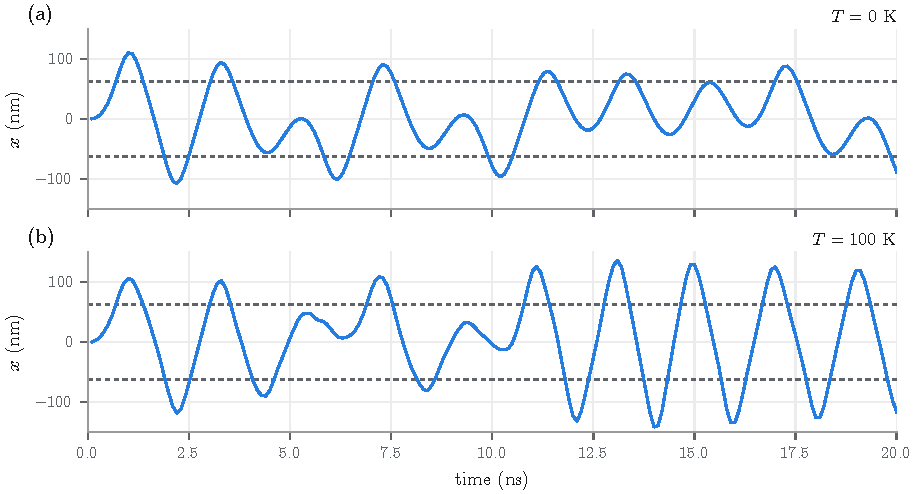
\includegraphics[width=\textwidth]{figures/driven_dw.pdf}
\caption{Position of a DW between two anti-notches in a $400\times50\times5$~nm Ni wire, driven by a 990~A/m, 500~MHz field (shipped \texttt{input}, RK4, $\Delta t=0.1$~ps), starting at the barrier top $x=0$. (a)~At 0~K the motion is deterministic: the DW crosses the barrier between the two wells in an irregular sequence. (b)~At 100~K, with the same initial state, thermal noise changes the sequence of crossings after the first few periods. Dashed lines: minima of the pinning potential at $\pm63$~nm.}
\label{fig:driven}
\end{figure}

\section{Ni nanowire under a femtosecond laser pulse}\label{sec:ni}
Beaurepaire's Ni TTM parameters~\cite{beaurepaire}, Evans' $M_s(T)$ for Ni~\cite{evans2015}, and the absorbed energy density of a 7~mJ/cm$^2$, 60~fs pulse on a 22~nm Ni film with about 35\% absorption ($1.13\times10^9$~J/m$^3$), applied to the $400\times50\times5$~nm wire. \key{Ms} and \key{Aex} are the 0~K values that give 477~kA/m and $1.05\times10^{-11}$~J/m at 300~K; $C_l$ is the bulk Ni value. Keys that differ from the shipped input:
\begin{lstlisting}
Ms=509407.45
Aex=1.19752e-11
Temperature=300
use_Ms_T=1
Tc=635
Ms_exponent=0.341
Ms_rescaling_exponent=2.322
Aex_exponent=2
pinning_exponent=2
use_TTM=1
TTM_gamma_e=6e3
TTM_C_l=3.9e6
TTM_G=8e17
TTM_P0=1.76356e22
TTM_t0=0.5e-12
TTM_sigma=2.548e-14
TTM_tau_m=200e-15
Dt=5e-17
totaltime=5.5e-12
out_time=1e-15
\end{lstlisting}
$T_e$ peaks at 676~K about 70~fs after the pulse maximum and stays above $T_c$ for roughly 0.7~ps (Figure~\ref{fig:ttm}). $M_s$ falls to 3.2\% of its 300~K value with $\tau_m=200$~fs and to 10\% with $\tau_m=300$~fs, then recovers towards the equilibrium of the heated lattice. With \key{TTM_tau_m=100e-15} the same pulse demagnetises the wire completely and the run stops.

\begin{figure}[!htb]\centering
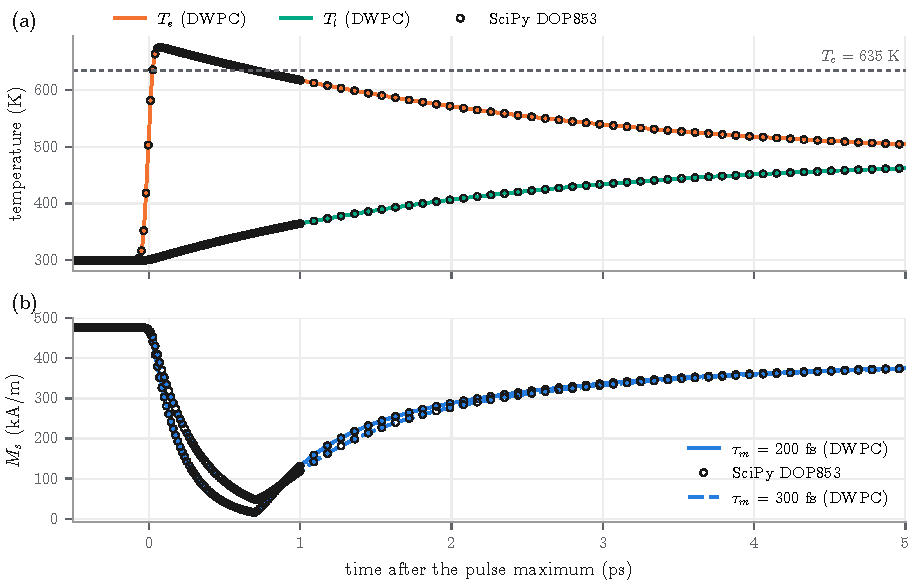
\includegraphics[width=\textwidth]{figures/ttm_ni.pdf}
\caption{Ni wire heated by a 60~fs (FWHM) pulse that deposits $1.13\times10^{9}$~J/m$^3$, starting from 300~K; time is measured from the pulse maximum. (a)~Electron temperature $T_e$ (orange) and lattice temperature $T_l$ (green) from the two-temperature model in \dwpc{} (lines), with the independent SciPy DOP853 solution (circles, sparser after 1~ps). $T_e$ peaks at 676~K, above $T_c=635$~K (dashed), and the two baths approach each other over several picoseconds. (b)~Saturation magnetisation for the relaxation times $\tau_m=200$~fs (solid) and 300~fs (dashed), with the SciPy solutions (circles). $M_s$ falls to 3.2\% and 10\% of its 300~K value, respectively, and then recovers towards $M_s(T_l)$. The largest deviation between \dwpc{} and SciPy is $5\times10^{-7}$~K (Section~\ref{sec:ttmcheck}).}
\label{fig:ttm}
\end{figure}

\section{Three coupled wires}
\begin{lstlisting}
Nwires=3
use_DW_coupling=1
rij=50e-9
program=Benchmark3
integrator=RK4
rng_seed=12345
\end{lstlisting}
\texttt{Benchmark3.data} holds $x$ and $\phi$ of each wire. Add the keys of Section~\ref{sec:ni} to excite all three wires with the same pulse. To compare runs with and without the pulse, keep \key{rng_seed} fixed and switch \key{use_TTM} between 1 and 0: the two runs share the same noise and coincide exactly until the pulse.

\section{Ensembles on a Slurm cluster}\label{sec:cluster}
The \texttt{cluster/} folder automates paired runs (same seed, with and without the pulse):
\begin{lstlisting}
bash cluster/deploy.sh                       # copy and build DWPC on every node
sbatch --array=1-100 cluster/dwpc_ensemble.sbatch
NSEED=100 sbatch --array=0-799 cluster/dwpc_distance_scan.sbatch
bash cluster/collect.sh                      # SRC=dwpc_scan for the scan
python3 cluster/analyze.py ~/dwpc_ens_all
python3 cluster/analyze_scan.py ~/dwpc_scan_all
\end{lstlisting}
All physics parameters of these runs live in \texttt{cluster/make\_input.sh}. The analysis scripts compute $\Delta x=x_{\rm laser}-x_{\rm ref}$ per wire and seed, its mean, standard error and $t$-statistic, and (for the scan) the Pearson correlation of $\Delta x$ between wires with 95\% confidence intervals.

%======================================================================
\chapter{Reservoir computing tasks}\label{ch:rc}

\dwpc{} ships two benchmark tasks that use a single DW as a physical reservoir~\cite{ababei2021}: the classification of sine and square waves (\key{program=RC}) and the recognition of spoken digits (\key{program=spoken_digit_recognition}). Both use one wire (\key{Nwires=1}), the integrator \texttt{integrate::runge\_kutta} (RK4, with thermal noise when \key{Temperature}~$>0$) and all physical parameters of \texttt{input}. The task settings are read from \texttt{rc\_input} (Section~\ref{sec:rcinput}). This chapter describes what the code does, how to run each task and what it gives with the shipped data.

\section{The DW as a reservoir node}\label{sec:rcnode}
In both tasks the input changes the amplitude of the driving field. The applied field is
\begin{equation}
H(t) = V_0\,\sin(2\pi f t), \qquad V_0 = H_0 + dH\,\tilde u ,
\label{eq:rcfield}
\end{equation}
where $f$ is the key \key{f} of \texttt{input} (500~MHz in the shipped file), $H_0$ and $dH$ are \key{H0} and \key{dH} of \texttt{rc\_input}, and $\tilde u$ is the (masked) input value. $V_0$ is held for one node time $\theta = T/N_v$ (\key{T}, \key{Nv}), during which the equations of motion are integrated for $n=\theta/\Delta t$ steps. The node state is a root-mean-square DW position over that window,
\begin{equation}
s = \Big(\tfrac{1}{n}\textstyle\sum_{j=1}^{n} x_j^2\Big)^{1/2}\quad(\text{nm}).
\label{eq:rcstate}
\end{equation}
The DW is not reset between nodes, so each state depends on the recent input history (fading memory) and on the nonlinear response of the double-well potential. Because $s$ depends on $x^2$, a DW that oscillates between the two wells gives the same state in the two half-cycles of the drive; with $\theta = 0.5$~ns and $f=500$~MHz this produces the alternation between two levels seen in Figs.~\ref{fig:rcsine} and~\ref{fig:rcspoken}.

The readout is linear, without a bias term. With the states of all samples in the matrix $\mathbf S$ (one row per sample) and the targets in $\mathbf Y$, the weights solve the ridge-regularised normal equations
\begin{equation}
\left(\mathbf S^{\mathsf T}\mathbf S + \alpha^2\mathbf I\right)\mathbf W^{\mathsf T} = \mathbf S^{\mathsf T}\mathbf Y ,
\label{eq:ridge}
\end{equation}
using LAPACK \texttt{dgesv} (sine/square) or \texttt{dgelss} (spoken digits, singular values below $10^{-10}$ of the largest are discarded). The prediction for a sample with state $\mathbf s$ is $\mathbf W\mathbf s$.

\section{Sine/square classification}\label{sec:rcsine}
\paragraph{Task.} The file \texttt{sine\_square\_init} has two columns, the input $u_k$ and the label $y_k$, and 1280 rows: 80 blocks of 16 samples, each block one period of a sine ($u_k=\sin(2\pi k/16)$) or a square wave ($\pm1$). The label is 1 for square-wave samples and 0 for sine samples. The values $u=\pm1$ occur in both classes, so the class of a sample cannot be read from the current input alone: the reservoir must supply memory of the previous samples. A linear readout of $u_k$ itself (with a bias) gives only the majority class.

\paragraph{Algorithm.} Implemented in \texttt{reservoir::run} and \texttt{batch\_training} in \texttt{src/rc.cpp}.
\begin{enumerate}
\item Draw a mask $m_i\in\{-1,+1\}$, $i=1\dots N_v$, from \key{seed}; the same mask is used for every sample.
\item Split the data: the first half (640 samples) is the training set, the second half the validation set.
\item For every sample $k$ and node $i$, set $V_0 = H_0 + dH\,(0.001 + u_k)\,m_i$, integrate for $\theta$ and store $s_{ki}$ from Eq.~\eqref{eq:rcstate}. The simulation time runs on through the whole set, and starts again from zero (with the DW state kept) for the validation set.
\item Solve Eq.~\eqref{eq:ridge} with $N_{\rm out}=1$ and $\alpha=0.001$ (hard-coded; \key{lambda} is not used by this task).
\item Classify a sample as square when $\mathbf W\mathbf s_k>0.5$; report the number of correct samples in both sets.
\end{enumerate}

\paragraph{Running it.}
\begin{lstlisting}
# input:     program=RC   (plus the physical parameters)
# rc_input:  file=sine_square_init
#            T=5e-9  Nv=10  H0=2280  dH=1500  seed=27256
cp sine_square_init run/ ; cd run ; ../dwpc
\end{lstlisting}
The task uses \key{file}, \key{T}, \key{Nv}, \key{H0}, \key{dH} and \key{seed}. It also reads \key{lr}, \key{la} and \key{Ne}, but the gradient-descent readout that used them is commented out. Note that the shipped \texttt{rc\_input} points to \texttt{sine\_square\_new}, a four-column file used by other programs: \key{RC} reads its input two numbers at a time, so it would pair the columns wrongly. Use \texttt{sine\_square\_init}.

\paragraph{Output.} The weights and the two counts are printed on the screen (\texttt{Number correct = \dots} and \texttt{Validation: Number correct = \dots}). \texttt{Signal.out} and \texttt{Valid\_\allowbreak Signal.out} hold the states $s_{ki}$ of the two sets on a single line, sample after sample ($N_v$ values per sample, tab-separated); \texttt{field\_\allowbreak map.data} holds the validation count. A commented block in \texttt{run()} scans $H_0$ and $dH$ and writes the count for each pair to \texttt{field\_\allowbreak map.data}.

\paragraph{Results.} Table~\ref{tab:rcsine} gives the result with the shipped \texttt{input} and \texttt{rc\_input} ($\Delta t = 0.1$~ps, 5000 steps per node, $6.4\times10^7$ RK4 steps, 41~s on one core) at 0~K and 100~K. The weights recomputed from \texttt{Signal.out} with NumPy reproduce both counts exactly. Fig.~\ref{fig:rcsine} shows the first 160 training samples. At 0~K the readout separates the two classes except near the peaks of the sine, where the input is $\pm1$ as in a square wave. At 100~K the thermal noise of the DW position spreads the node states and the accuracy drops, most of all on the validation set.

\begin{table}[!htb]\centering\small
\caption{Sine/square classification with the shipped parameters ($T=5$~ns, $N_v=10$, $H_0=2280$~A/m, $dH=1500$~A/m, seed 27256, $\Delta t=0.1$~ps, RK4). Each set has 640 samples. The majority-class baseline assigns every sample to the more frequent class.}\label{tab:rcsine}
\begin{tabular}{@{}lcc@{}}\toprule
 & Training & Validation\\\midrule
Squares in the set & 240 & 368\\
Majority-class baseline & 400 (62.5\%) & 272 (42.5\%)\\
DW reservoir, 0~K & 565 (88.3\%) & 589 (92.0\%)\\
DW reservoir, 100~K & 481 (75.2\%) & 430 (67.2\%)\\\bottomrule
\end{tabular}
\end{table}

\begin{figure}[!htb]\centering
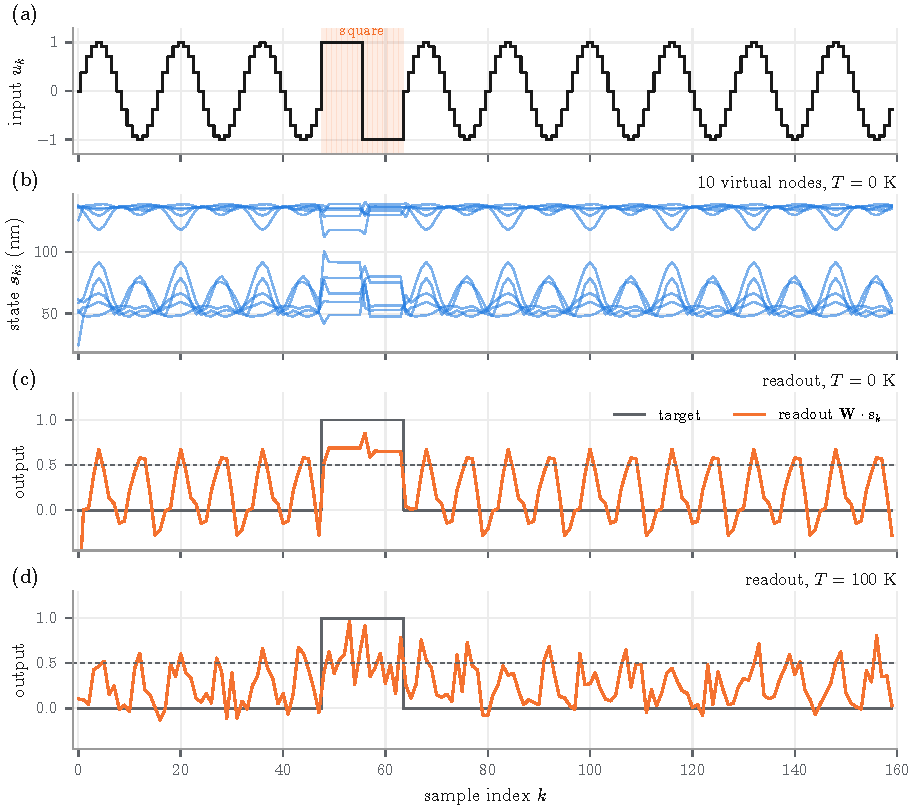
\includegraphics[width=\textwidth]{figures/rc_sine.pdf}
\caption{Sine/square classification, first 160 training samples (10 periods). (a)~Input $u_k$; the shaded block is a square-wave period (target 1), all others are sine periods (target 0). (b)~The ten virtual-node states $s_{ki}$ at 0~K, i.e.\ the RMS DW position over each node time $\theta=0.5$~ns; the two groups of curves come from the two signs of the mask. (c)~Linear readout $\mathbf W\cdot\mathbf s_k$ at 0~K (orange) with the target (gray) and the decision threshold 0.5 (dashed): the square period is detected, and the errors occur at the peaks of the sine, where the input equals $\pm1$ as in a square wave. (d)~Same at 100~K: thermal noise spreads the readout and the accuracy drops. Data: \texttt{Signal.out} of the two runs in Table~\ref{tab:rcsine}; the readout recomputed from these states reproduces the counts printed by \dwpc{}.}\label{fig:rcsine}
\end{figure}

\section{Spoken digit recognition}\label{sec:rcspoken}
\paragraph{Data.} The directory \texttt{spoken\_\allowbreak digit\_\allowbreak files} holds the files \texttt{Jackson.dat}, \texttt{Nicolas.dat}, \texttt{Theo.dat} and \texttt{Yweweler.dat}, one per speaker, each with 500 rows: 50 utterances of each digit 0--9, sorted by digit. According to \texttt{README.docx} in that directory, each row is a filtered spectrogram with 64 frequency channels and 16 time steps, written as 1024 values with the 16 time steps of the first channel first, followed by the digit in column 1025. The input values lie between 0 and 0.82.

\paragraph{Algorithm.} Implemented in \texttt{run\_\allowbreak spoken\_\allowbreak recognition}, \texttt{spoken\_\allowbreak training} and \texttt{get\_\allowbreak signal\_\allowbreak digit}.
\begin{enumerate}
\item Read 2000 rows of 1025 numbers from \texttt{Signal\_in.data} in the run directory (the size is hard-coded).
\item For each utterance $i$, set $x=0$ and $t=0$ ($\phi$ is kept from the previous utterance). For each feature $k=1\dots1024$, set $V_0 = H_0 + dH\,u_{ik}$ (no mask), integrate for $\theta=T/N_v$ and store $X_{ik} = \big(\sum_j x_j^2\big)^{1/2}/16$. Each feature is one node; $N_v$ only sets $\theta$. The factor $1/16$ is left over from an earlier version that averaged 16 time steps, so $X$ scales as $\sqrt{\theta/\Delta t}$, and the effective strength of the regularisation changes with $\Delta t$.
\item Encode the labels one-hot ($N_{\rm out}=10$), solve Eq.~\eqref{eq:ridge} with $\alpha=$ \key{lambda} and predict the digit with the largest output.
\item Report the number of correct predictions on the same 2000 utterances. There is no held-out set in the C++ code.
\end{enumerate}

\paragraph{Running it.}
\begin{lstlisting}
cd run
cat ../spoken_digit_files/{Jackson,Nicolas,Theo,Yweweler}.dat > Signal_in.data
# input:     program=spoken_digit_recognition
# rc_input:  T=5e-9  Nv=10  H0=2280  dH=1500  lambda=2.1  seed=27256
../dwpc > log
\end{lstlisting}
The task uses \key{T}, \key{Nv}, \key{H0}, \key{dH}, \key{lambda} and \key{seed} (the mask is drawn but not used).

\paragraph{Output.} \texttt{Processed\_\allowbreak spoken\_\allowbreak signal.txt} holds the $2000\times1024$ feature matrix $X$. The screen output contains the mean-squared error of the readout, the $2000\times10$ prediction matrix, one line per utterance (index, true digit, predicted digit, largest target, largest output) and \texttt{No of correct predictions: \dots}.

\paragraph{Held-out evaluation.} The scripts \texttt{split.sh} and \texttt{Spoken\_\allowbreak Classification.py} in \texttt{spoken\_\allowbreak digit\_\allowbreak files} evaluate the features on unseen data. \texttt{split.sh} cuts \texttt{Processed\_\allowbreak spoken\_\allowbreak signal.txt} into blocks of 50 lines (one digit of one speaker), puts the first 25 utterances of each block in \texttt{Training.data} and the last 25 in \texttt{Validation.data}, and does the same with the one-hot labels in \texttt{Y\_vec.txt}. The current code does not write \texttt{Y\_vec.txt}; make it from column 1025 of \texttt{Signal\_in.data}. \texttt{Spoken\_\allowbreak Classification.py} then solves Eq.~\eqref{eq:ridge} on the training half and counts the correct predictions on the validation half.

\paragraph{Readout bug (fixed).} Until this version the readout returned 200 correct out of 2000, the chance level: every utterance was assigned to the digit 4. The right-hand side $\mathbf S^{\mathsf T}\mathbf Y$ was stored row by row ($N\times N_{\rm out}$), while LAPACK reads it column by column, so for $N_{\rm out}>1$ the ten target columns were mixed before the solve. The fix stores the right-hand side as an $N_{\rm out}\times N$ array, which is the column-major layout LAPACK expects, in all three regression routines (the sine/square task, with $N_{\rm out}=1$, was not affected). With the same features the corrected readout gives 1971 out of 2000, identical to an independent NumPy solution. The mean-squared error is now computed against the targets instead of the features, and \texttt{spoken\_training} returns the count.

\paragraph{Results.} Table~\ref{tab:rcspoken} gives the result with the shipped \texttt{rc\_input} ($T=5$~ns, $N_v=10$, so $\theta=0.5$~ns per feature) and $\Delta t = 1$~ps (500 steps per feature, $1.0\times10^9$ RK4 steps, about 10~min on one core for the features and 30~s for the readout). The in-sample count is the number the program prints. The held-out counts use the 25/25 split of \texttt{split.sh}, the leave-one-speaker-out (LOSO) counts train on three speakers and test on the fourth; both use Eq.~\eqref{eq:ridge} on the features from \texttt{Processed\_\allowbreak spoken\_\allowbreak signal.txt}, with the $\alpha$ that gives the best held-out count among $10^{-3},10^{-1},1,2.1,10,10^2,10^3,10^4$. The last row applies the same readout to the input values $u_{ik}$ themselves, without the DW. Fig.~\ref{fig:rcspoken} shows the features of one utterance and the confusion matrix of the held-out set at 0~K.

\begin{table}[!htb]\centering\small
\caption{Spoken digit recognition, 4 speakers $\times$ 500 utterances, shipped \texttt{rc\_input}, $\Delta t=1$~ps, RK4. In-sample: trained and scored on all 2000 utterances with $\alpha=2.1$ (the number printed by \dwpc). Held-out: 1000 training and 1000 test utterances. LOSO: sum over the four speakers of the correct predictions on the speaker left out (500 each).}\label{tab:rcspoken}
\begin{tabular}{@{}lcccc@{}}\toprule
Features & In-sample & Held-out & $\alpha$ & LOSO\\\midrule
DW reservoir, 0~K & 1999/2000 & 841/1000 (84.1\%) & 100 & 1524/2000 (76.2\%)\\
DW reservoir, 100~K & 1971/2000 & 264/1000 (26.4\%) & 100 & 580/2000 (29.0\%)\\
Input values, no DW & -- & 879/1000 (87.9\%) & 2.1 & 1645/2000 (82.3\%)\\\bottomrule
\end{tabular}
\end{table}

\begin{figure}[!htb]\centering
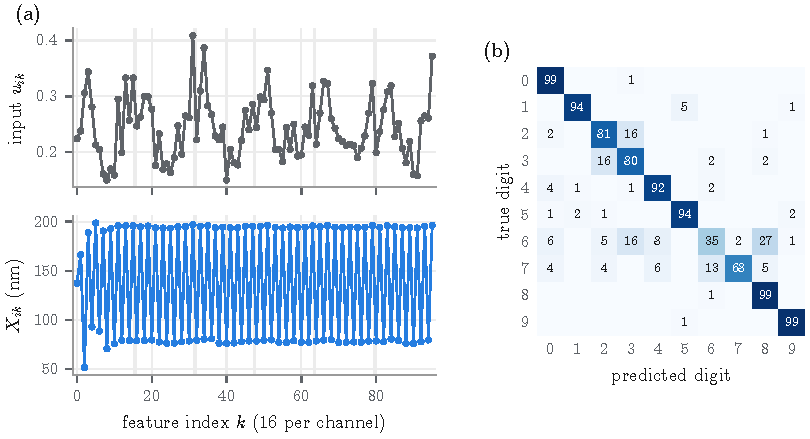
\includegraphics[width=\textwidth]{figures/rc_spoken.pdf}
\caption{Spoken digit recognition at 0~K. (a)~Top: the first 96 input values of one utterance of ``3'' by Jackson, i.e.\ the 16 time steps of the first six frequency channels (vertical lines separate the channels). Bottom: the corresponding DW features $X_{ik}$; their alternation between two levels comes from sampling the 500~MHz drive in windows of a quarter period, and the input modulates the levels. (b)~Confusion matrix of the held-out test set (25 utterances per digit and speaker, 1000 in total) for a ridge readout with $\alpha=100$ trained on the other 1000 utterances: 841 correct. The main confusions are 2$\leftrightarrow$3, 6$\to$8 and 6$\to$3, and 7$\to$6. Data: \texttt{Processed\_\allowbreak spoken\_\allowbreak signal.txt} of the 0~K run in Table~\ref{tab:rcspoken}.}\label{fig:rcspoken}
\end{figure}

The in-sample counts are close to 100\% in every case because the readout has 1024 weights per digit for 2000 utterances; they do not measure generalisation and should not be quoted as the accuracy of the reservoir. On unseen utterances, the DW features at 0~K reach 84\% (held-out) and 76\% (LOSO); most errors are between 2 and 3 and for the digits 6 and 7. A linear readout of the raw input does slightly better with these parameters. At 100~K the thermal noise dominates the features and the held-out accuracy falls to 26\%. The shipped parameters have therefore not been optimised for the current version of the model (which also includes the corrected demagnetising factors, Section~\ref{sec:demag}). Before claiming a benefit from the DW, scan $H_0$, $dH$, $\theta$ and $f$, add a mask over several virtual nodes per feature, and always report a held-out or LOSO score next to the raw-input baseline.

\section{Checklist}
\begin{itemize}
\item Sine/square: \texttt{file=sine\_square\_init}; the counts on the screen are the result. \key{lambda}, \key{lr}, \key{la} and \key{Ne} have no effect.
\item Spoken digits: build \texttt{Signal\_in.data} from the four speaker files; the printed count is in-sample. Use \texttt{split.sh} and \texttt{Spoken\_\allowbreak Classification.py} (or a LOSO split) for the accuracy on unseen data.
\item The number of RK4 steps is $\theta/\Delta t$ per node. At $\Delta t = 0.1$~ps the spoken-digit task needs $10^{10}$ steps (about 100~min on one core); $\Delta t = 1$~ps is ten times faster, but it changes the scale of the features and therefore the effective regularisation.
\item Both tasks use the thermal noise of \key{Temperature}; set it to 0 to separate the deterministic response from the noise.
\end{itemize}

%======================================================================
\chapter{Validity and limitations}\label{ch:limits}

\dwpc{} is a reduced model: it is fast because it ignores the internal structure of the wall.
\begin{center}\small
\begin{tabularx}{\textwidth}{@{}>{\raggedright}X >{\raggedright}X >{\raggedright\arraybackslash}X@{}}
\toprule Assumption & Fails when & Check with\\\midrule
Rigid transverse wall described by $x$ and $\phi$ & the wall tilts, changes type or nucleates new walls, e.g.\ near $T_c$ or above Walker breakdown & MuMax3 or VAMPIRE snapshots\\
Symmetric polynomial pinning ($a_2,a_4,a_6$ only) & the real notch is asymmetric or the DW leaves the fitted range & refit $E(x)$ over the explored range\\
Point-charge coupling, nearest neighbours & centre distance below a few wire widths, or many wires at small spacing & micromagnetic interaction energy vs.\ distance\\
Constant dipole moment $m_y$ & $M_s$ changes with temperature & to be fixed in the code\\
Single-time relaxation of $M_s$ ($\tau_m$) & ultrafast demagnetisation matters quantitatively & atomistic $m(t)$ (VAMPIRE TTM runs)\\
$A\propto M_s^n$, $E_{\rm pin}\propto M_s^p$ with chosen $n,p$ & exponents differ from the assumed values & atomistic or micromagnetic $A(T)$ and pinning\\
Uniform heating over the thickness & absorption depth smaller than $L_z$ & optical model, or $P_0$ instead of fluence\\
\bottomrule
\end{tabularx}
\end{center}

% Known issues: hidden from the PDF. Change \iffalse to \iftrue to show them again.
\iffalse
\section{Known issues}\label{sec:issues}
\begin{itemize}
\item \key{EULER} does not evaluate the applied field (the stored field is never updated), the noise, the spin torque or the coupling: a DW started at the barrier top stays at rest. Do not use it.
\item \texttt{calculate::current()} returns a value proportional to $j^2$ for a single DW.
\item \key{RK45} contains no thermal noise.
\item The single-DW initial position is fixed at $x=0$, the top of the barrier; only multi-wire runs accept \key{DW_x0_<i>}.
\item \key{H_const} is switched off after 25~ns and \key{Bifurcation} ignores \key{H}; both are hard-coded.
\item The noise uses \texttt{std::default\_random\_engine} (\texttt{minstd\_rand0} with g++); use a stronger generator such as \texttt{std::mt19937\_64} before any statistical test of randomness.
\item The Lyapunov estimate does not renormalise the separation.
\item Three functions declared to return \texttt{double} end without a return statement (undefined behaviour at \texttt{-O3}), and the code builds with about 70 warnings under \texttt{-Wall -Wextra}.
\item Results before commit \texttt{dd3d90c} used $\log_{10}$ in the demagnetising factors.
\item Before this version the spoken-digit readout mixed the ten target columns (row- versus column-major storage for LAPACK) and returned the chance level, 200 of 2000; see Section~\ref{sec:rcspoken}.
\item The spoken-digit program scores its readout on the training data only, the feature scale depends on $\Delta t$, and the file size (2000 rows) is hard-coded. The shipped \texttt{rc\_input} points \key{RC} to the four-column \texttt{sine\_square\_new}; use \texttt{sine\_square\_init}.
\end{itemize}
\fi

%======================================================================
\begin{thebibliography}{99}
\bibitem{ababei2021} R.~V. Ababei, M.~O.~A. Ellis, I.~T. Vidamour, D.~S. Devadasan, D.~A. Allwood, E.~Vasilaki and T.~J. Hayward, \emph{Neuromorphic computation with a single magnetic domain wall}, Sci.\ Rep.\ \textbf{11}, 15587 (2021). \url{https://doi.org/10.1038/s41598-021-94975-y}
\bibitem{ababei2026} R.-V. Ababei, \emph{Atomistic origin of nonlinear bistable domain wall dynamics in double-notched Ni nanowires}, J.\ Magn.\ Magn.\ Mater.\ \textbf{655}, 174399 (2026). \url{https://doi.org/10.1016/j.jmmm.2026.174399}
\bibitem{malozemoff} A.~P. Malozemoff and J.~C. Slonczewski, \emph{Magnetic Domain Walls in Bubble Materials} (Academic Press, 1979).
\bibitem{thiaville} A.~Thiaville, Y.~Nakatani, J.~Miltat and Y.~Suzuki, Europhys.\ Lett.\ \textbf{69}, 990 (2005).
\bibitem{aharoni} A.~Aharoni, J.\ Appl.\ Phys.\ \textbf{83}, 3432 (1998).
\bibitem{brown} W.~F. Brown, Phys.\ Rev.\ \textbf{130}, 1677 (1963).
\bibitem{obrien} L.~O'Brien \emph{et al.}, Phys.\ Rev.\ Lett.\ \textbf{103}, 077206 (2009).
\bibitem{hayward} T.~J. Hayward \emph{et al.}, \emph{Pinning induced by inter-domain wall interactions in planar magnetic nanowires}. \url{https://escholarship.org/uc/item/8kq537ft}
\bibitem{pivano} A.~Pivano and V.~O. Dolocan, \emph{Chaotic dynamics of magnetic domain walls in nanowires}, arXiv:1604.04438.
\bibitem{beaurepaire} E.~Beaurepaire, J.-C. Merle, A.~Daunois and J.-Y. Bigot, Phys.\ Rev.\ Lett.\ \textbf{76}, 4250 (1996).
\bibitem{evans2015} R.~F.~L. Evans, U.~Atxitia and R.~W. Chantrell, Phys.\ Rev.\ B \textbf{91}, 144425 (2015).
\bibitem{ababei2024} R.-V. Ababei, R.~F.~L. Evans, M.~Agop and R.~W. Chantrell, Phys.\ Rev.\ B \textbf{109}, 094437 (2024).
\bibitem{binh} N.~T. Binh, S.~Ruta, O.~Hovorka, R.~F.~L. Evans and R.~W. Chantrell, Phys.\ Rev.\ B, 054421 (2022).
\end{thebibliography}

\end{document}
